\documentclass[11pt]{article}
\usepackage[framemethod=TikZ]{mdframed}
\usepackage{amsthm}
\usepackage{tcolorbox}
\usepackage[margin=0.75in]{geometry}
\usepackage{setspace}
\usepackage{amsmath}
\usepackage{cancel}
\usepackage{multicol}
\def\deg{\ensuremath{^\circ}}
\def\v#1{\ensuremath{\mathrm{#1}}}
\usepackage{multirow}
\usepackage{fancyhdr}
\pagestyle{fancy}
\usepackage{lastpage} 
\usepackage{colortbl}
\usepackage{amssymb}
\usepackage{graphicx}
\setlength{\parskip}{0pt}
\lhead{Jhon Christian N. Rozano}
\chead{}
\rhead{May 5, 2021}

\lfoot{Source: Brilliant}
\cfoot{}
\rfoot{Page \thepage\ of \pageref{LastPage}}

\renewcommand{\headrulewidth}{1pt}

\renewcommand{\footrulewidth}{1pt}

\newcommand*\Eval[3]{\left.#1\right\rvert_{#2}^{#3}}

\definecolor{LightCyan}{rgb}{0.88,1,1}



\begin{document}
	\setlength{\columnsep}{10pt}
	\renewcommand{\arraystretch}{1.5}
	\singlespacing
	\newtcolorbox{mybox}[1]{title=#1}
	
	\begin{center}
		{\large  \textbf{Physics Problem of the Day}} \\ 
	\end{center}
	\begin{center}
	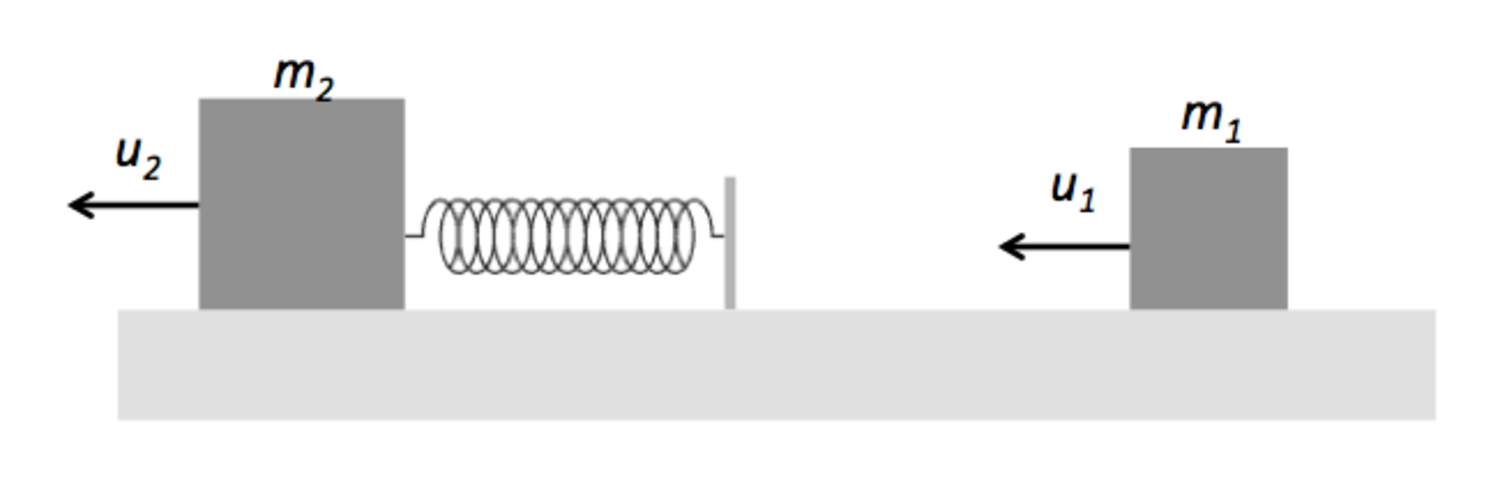
\includegraphics[clip=true, scale=0.2]{5b29986a80.56d979c1b5.j6ylFT}
	\end{center}
	
	\noindent A block of mass \( m_1 = 3\text{ kg} \) is moving on a frictionless horizontal surface with a velocity of \( u_1 = 16\text{ m/s} \) towards another block of mass \( m_2 = 9\text{ kg} \) that is moving on the same surface with a velocity of \( u_2 = 8\text{ m/s} \) in the same direction. A massless spring of spring constant \( k=36\text{ N/m} \) is attached to \( m_2 \) as shown in the figure above. When block \( m_1 \) collides with the spring, what is the maximum change in the spring's length?
	\\
	\begin{mybox}{\textbf{Solution}}
	Observe that as the box 1 collides with box 2, the maximum change in the spring's length could be calculated when the velocity of the two boxes is the same. The velocity can be calculated by the collision in linear momentum.
	\[ m_1u_1 + m_2u_2 = m_1u_f + m_2u_f = \left( m_1 + m_2 \right)u_f  \]
	\[ \Rightarrow \left( 3\text{ kg} \right) \times \left( 16\text{ m/s} \right) + \left( 9\text{ kg} \right) \times \left( 8\text{ m/s} \right) = \left( 3\text{ kg} + 9\text{ kg} \right)u_f \]
	\[ u_f = \frac{\left( 3\text{ kg} \right) \times \left( 16\text{ m/s} \right) + \left( 9\text{ kg} \right) \times \left( 8\text{ m/s} \right)}{3\text{ kg} + 9\text{ kg}} = \frac{120\text{ kg m/s}}{12\text{ kg}} = 10\text{ m/s} \]
	\\
	Therefore, the velocity of boxes 1 and 2, respectively, is \(10\text{ m/s} \). To compute for the maximum change in the spring's length, we will use the law of conservation of energy. Notice that the loss in the kinetic energy of the boxes will be the gain in the elastic potential energy of the spring. Thus, we have
	\\
	\[ \frac{1}{2}m_1{u_1}^2 + \frac{1}{2}m_2{u_2}^2 - \left(  \frac{1}{2}m_1{u_f}^2 + \frac{1}{2}m_2{u_f}^2 \right) = \frac{1}{2}k {\Delta x}^2  \]
	\[ \frac{1}{2}m_1{u_1}^2 + \frac{1}{2}m_2{u_2}^2 - \frac{1}{2}\left( m_1+m_2\right){u_f}^2  = \frac{1}{2}k {\Delta x}^2  \]
	\[ \frac{1}{2} \times (3\text{ kg}) \times {(16\text{ m/s})}^2 + \frac{1}{2} \times (9\text{ kg}) \times {(8\text{ m/s})}^2 - \frac{1}{2} (3\text{ kg}+9\text{ kg}){(10\text{ m/s})}^2  = \frac{1}{2}\times(36\text{ N/m}) {\Delta x}^2  \]
	\[ 72\text{ J} = (18\text{ N/m}) \times ({\Delta x}^2) \]
	\[ 4\text{ m}^2 = {\Delta x}^2 \Rightarrow \boxed{ \Delta x = 2\text{ m}} \]
	\\
	Therefore, the maximum change in the length of the spring is \textcolor{red}{2\text{ m}}.
	\end{mybox}
	
	
	
	
\end{document}
